\chapter{SYSTEM DESIGN}
\section{Flow chart}
\begin{figure}[!h]
	\centering
	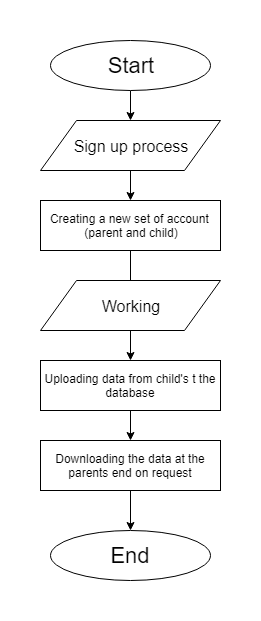
\includegraphics[height=7in]{flowchart.PNG}
	\caption{Flow chart}
\end{figure}

\section{Use case diagram}
\vspace{1in}
\begin{figure}[!h]
	\centering
	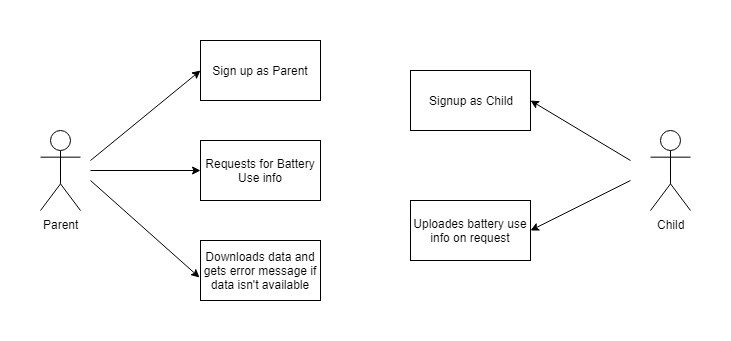
\includegraphics[height=3.4in]{UseCase.PNG}
	\caption{Use Case Diagram-}
\end{figure}
\newpage
\section{Activity Diagram}
\begin{figure}[!h]
	\centering
	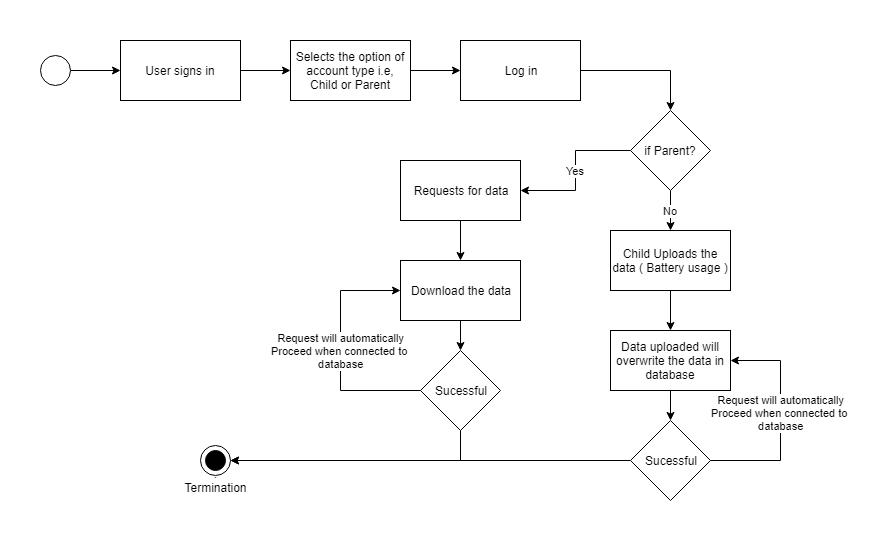
\includegraphics[height=4.5in]{Activity.PNG}
	\caption{Activity Diagram}
\end{figure}

\newpage
\chapter{IMPLEMENTATION}
\section{Introduction}
This project is basically a communication based application helpful of a family with busy guardians.It has a sign up functionality in which the new user can  sign up as “parent” or a “child” . the information regarding the usage of application of the child's phone will be uploaded and sent to database and then its been downloaded on the parent on request.

During the sign we ask for a “key” , it's nothing but a simple linking and deciding factor to bring together a set of parent and child. It helps establish a relationship between user, for example, a parent and its child will have a same key.
\begin{figure}[!h]
\centering
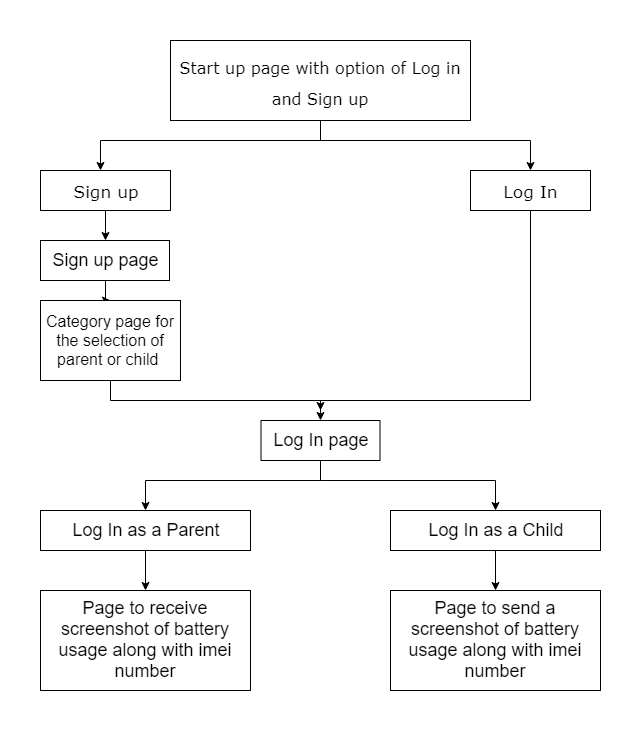
\includegraphics[height=5.3in]{flow.PNG}
\caption{Control flow in applicatition}
\end{figure}
\newpage
\section{Start up activity}
We will have two options here, If we sign up, it will direct us to sign up activity and then to category activity and further to login. Sign up activity helps us create and account (log in path) in the database and the we login after creation of account
\vspace{2cm}
\begin{figure}[!h]
	\centering
	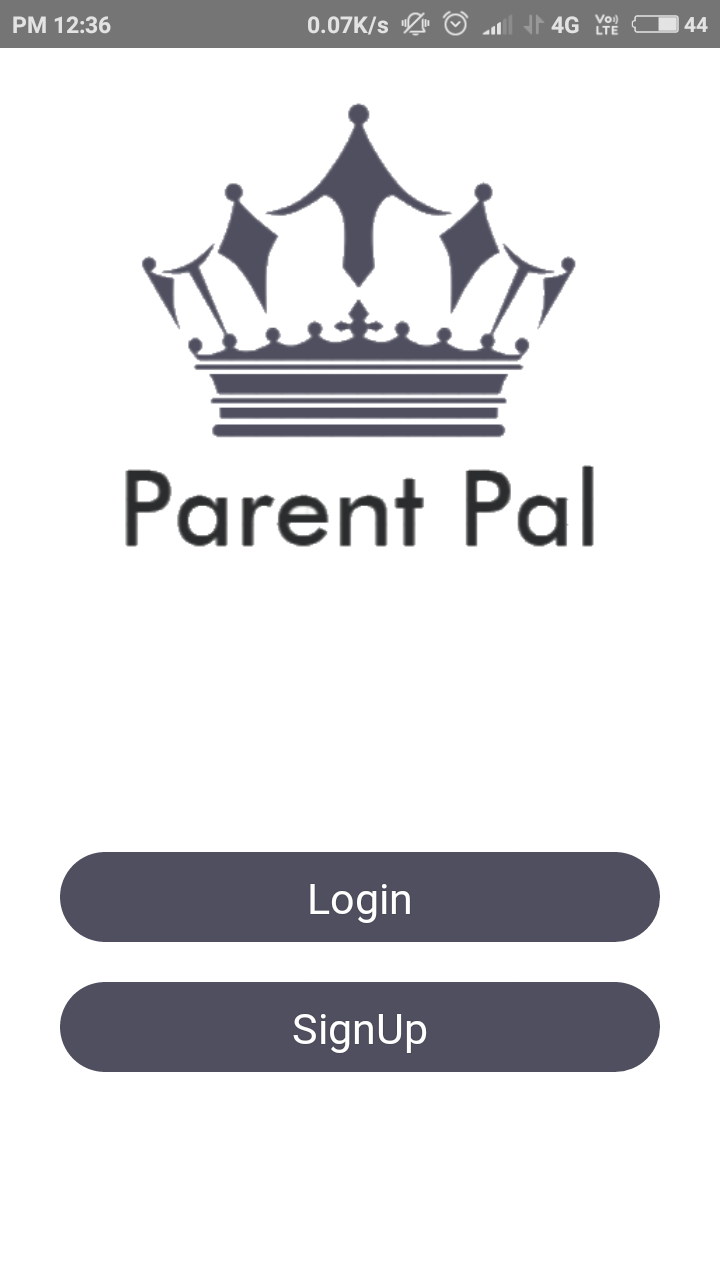
\includegraphics[height=7.3in]{Startup.PNG}
	\caption{Start up activity}
\end{figure}
\newpage

\section{Sign up sctivity}
Onclick of Sign up action button , it stores the value andredirects to another activity in which we select the type of account.
\begin{figure}[!h]
	\centering
	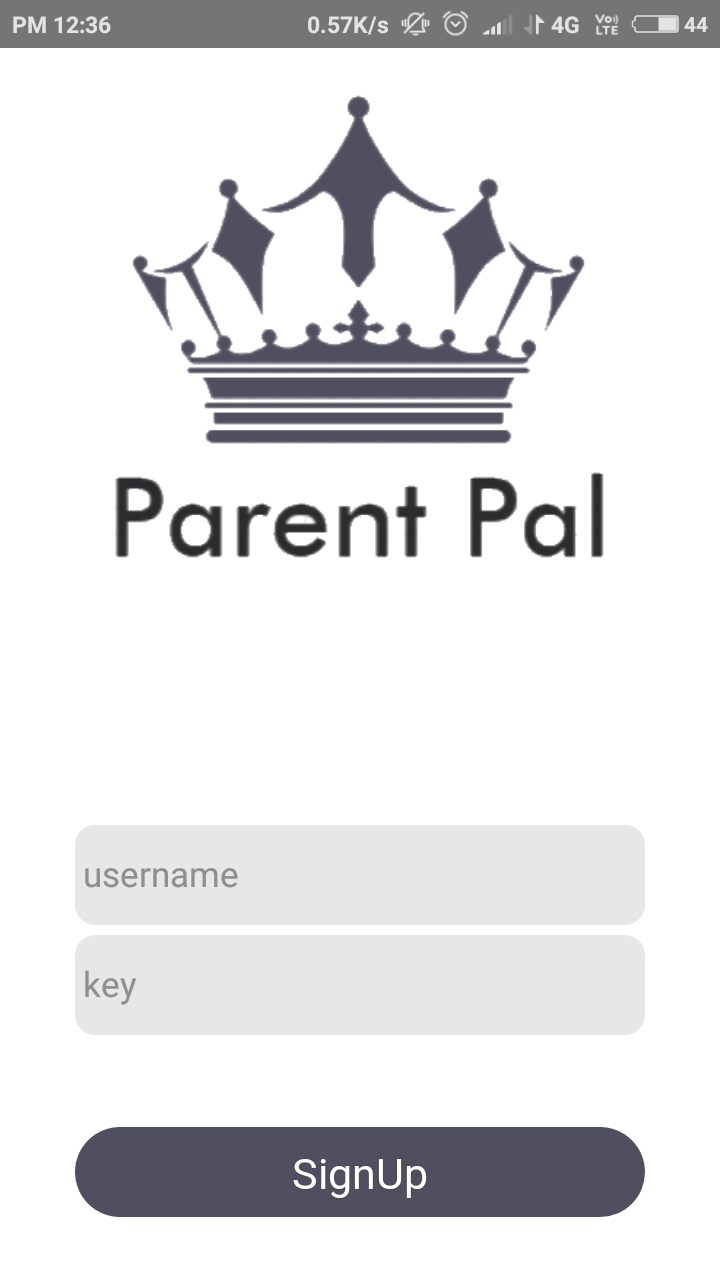
\includegraphics[height=7.3in]{Signup.PNG}
	\caption{Sign up activity}
\end{figure}
\newpage
\section{Log in activity}
On click of log in action button , it redirects according to the type of account.It redirect to a activity which allows us to upload data (if the account type is of child) or redirects to an activicy where can download the data (if the account type is or parent) .
\begin{figure}[!h]
	\centering
	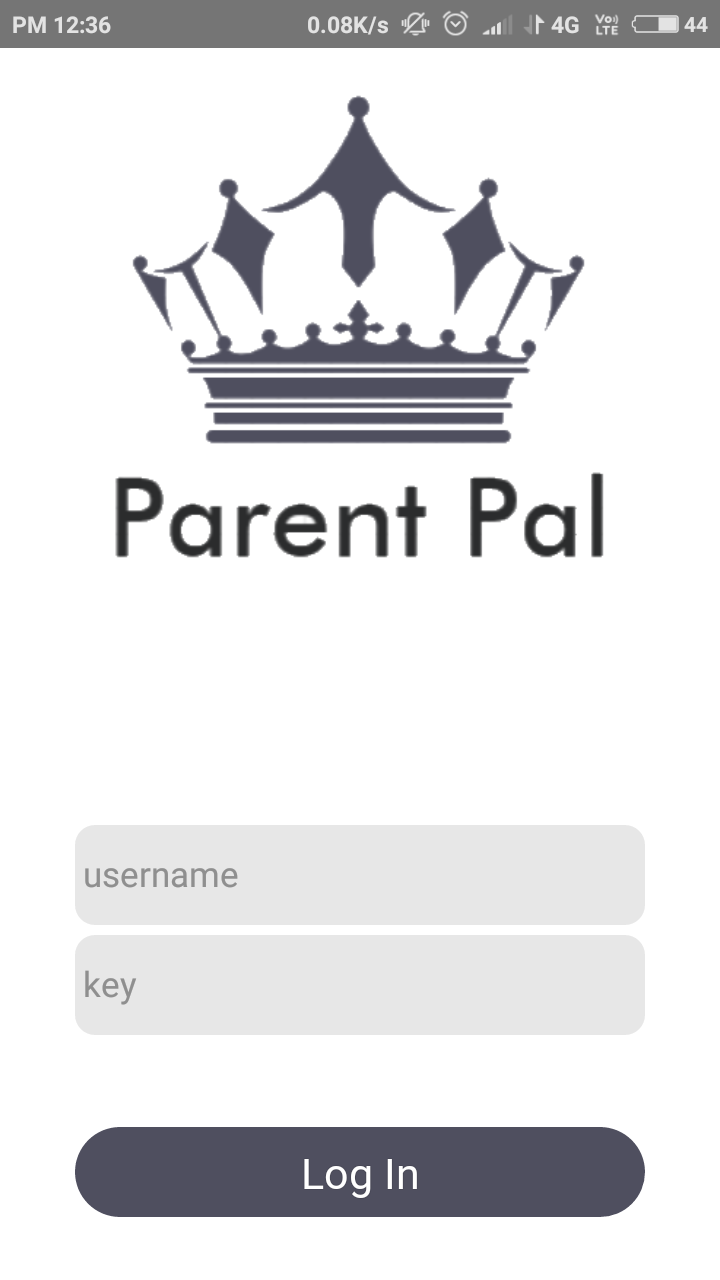
\includegraphics[height=7.3in]{Login.PNG}
	\caption{Log in activity}
\end{figure}
\newpage

\section{Category activity}
Helps us select the type of Account
\begin{figure}[!h]
	\centering
	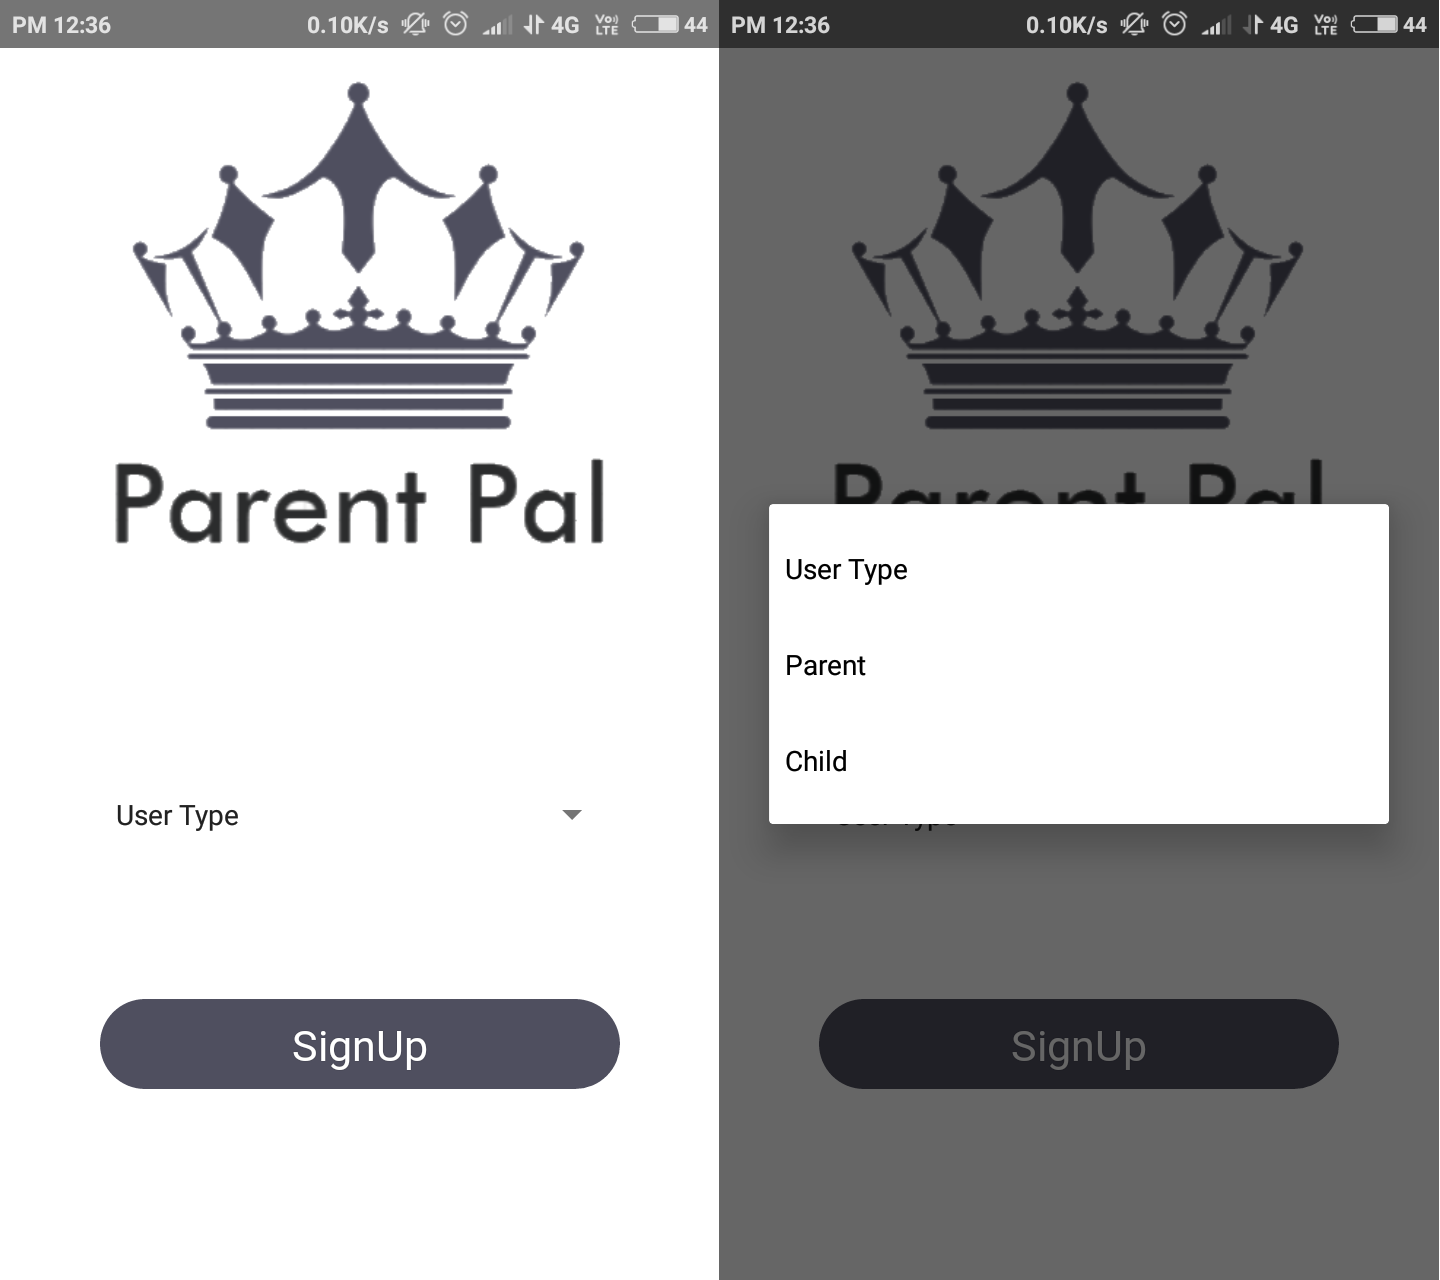
\includegraphics[height=6.3in]{catf.PNG}
	\caption{Category activity}
\end{figure}
\newpage
\section{Request activity}
For the reqest of uplaod or download
\begin{figure}[!h]
	\centering
	\includegraphics[height=7.3in]{Batuse.PNG}
	\caption{Request activity}
\end{figure}

\newpage
\chapter{RESULTS}
\section{Introduction}
Software testing is a critical element of software quality assurance and represents the ultimate review of specification, design and coding. In fact, testing is the one step in the software engineering process that could be viewed as destructive rather than constructive.
A strategy for software testing integrates software test case design methods into a well-planned series of steps that result in the successful construction of software. Testing is the set of activities that can be planned in advance and conducted systematically. The underlying motivation of program testing is to affirm software quality with methods that can economically and effectively apply to both strategic to both large and small-scale systems.

\section{Testing Objectives}
The main objective of performance testing is designed to test whether display is as expected and whether the webpage is functioning properly or not. 
As the test results are gathered and evaluated they begin to give a qualitative indication of the reliability of the code. If proper output is not obtained, the overall quality of the code is questioned. If, on the other hand, all the results which are not successful, are encountered, and are easily modifiable, then the following conclusion can be made: The tests are inadequate as the requirements mentioned are not compatible. The testing includes:
\begin{itemize}
	\item Checking whether the information is displayed or not.
	\item Checking whether all the players data is collected or not.
	\item Checking whether all the inputs are correctly taken or not.
	\item Verifying if all the pictures are displayed and none of the files are corrupted. 
\end{itemize}
\newpage

\section{Output screens}
Output is the battery use of the child's phone

\begin{figure}[!h]
\centering
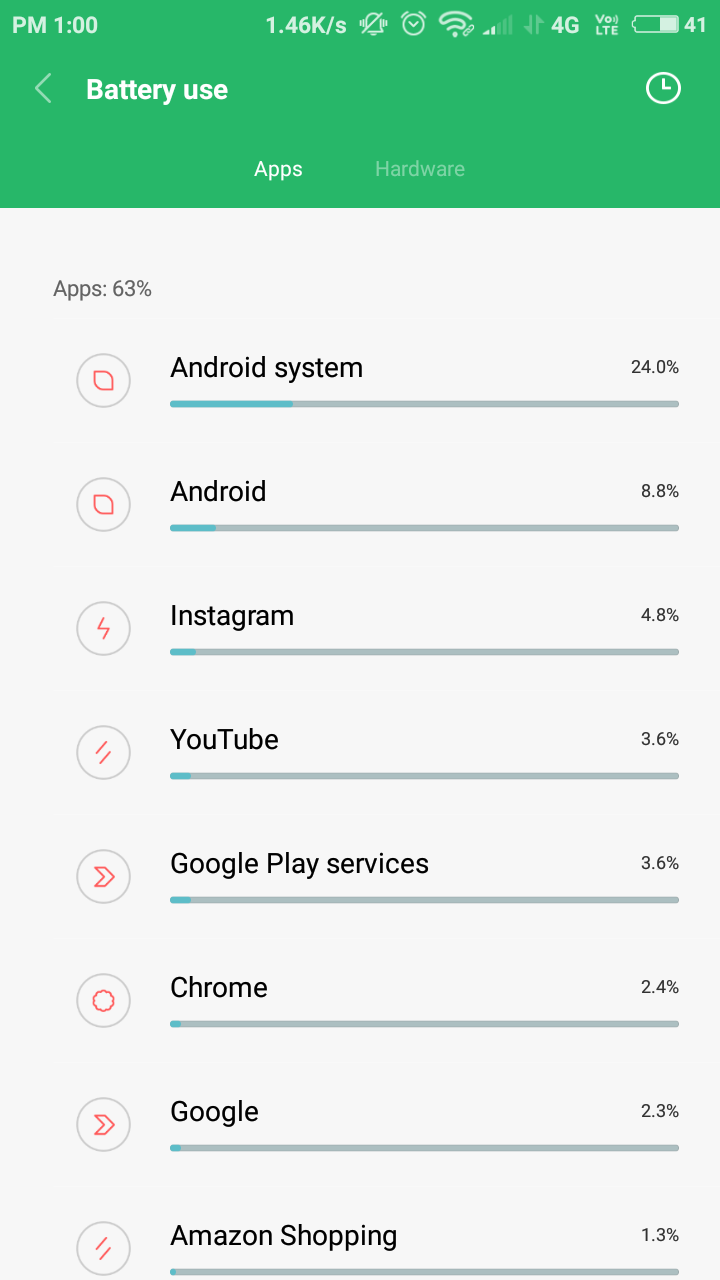
\includegraphics[height=7.5in]{out.PNG}
\caption{Output{\tiny }}
  
\end{figure}


\newpage


\chapter{CONCLUSION AND FUTURE SCOPE}

Overall we created an android (and ios) application using React-native which basically uploads and shares the battery use of a device. This was implemented on an android device and firebase.In future we will try to make it more advances by using live updates , background processes and remote control.This concept can also be used on other devices running on different platforms.



\newpage
\begin{thebibliography}{9}
\bibitem{react-native}
Text book
Mastering React Native by Eric Masiello 
\bibitem{bot}
RectJS tutorials
\\\texttt{https://www.tutorialspoint.com/reactjs/}

\bibitem{react-native}
React-native online documentataion and tutorials
\\\texttt{https://facebook.github.io/react-native/}
\bibitem{errors}
For debuggibg errors
\\\texttt{https://medium.com/}
\bibitem{bot}
For errors
\\\texttt{https://stackoverflow.com/}

\end{thebibliography}













